\documentclass[journal]{../IEEEtran}

\usepackage{graphicx}
\usepackage{fancyhdr}
\usepackage{epsfig} % for postscript graphics files
\usepackage{graphics} % for pdf, bitmapped graphics files

\pagestyle{fancy}
\lhead{CPE 470/670}
\rhead{\thepage}
\chead{Team 6: Lab 6 Report}
\lfoot{}
\rfoot{}
\cfoot{}

\begin{document}

\begin{titlepage}
    \vspace*{\fill}
    \begin{center}
      {\LARGE \bf Lab 6: Ball Sorting Contest}

      {Team 6: Alexander  C. Woods and Taylor Mansfield}

      November 5, 2014
    \end{center}
    \vspace*{\fill}
  \end{titlepage}


\section{Hardware and Software Design}\label{S.design}
\IEEEPARstart{L}{ine} following is a classic robotics problem

%\begin{figure}[ht]
%\centering
% 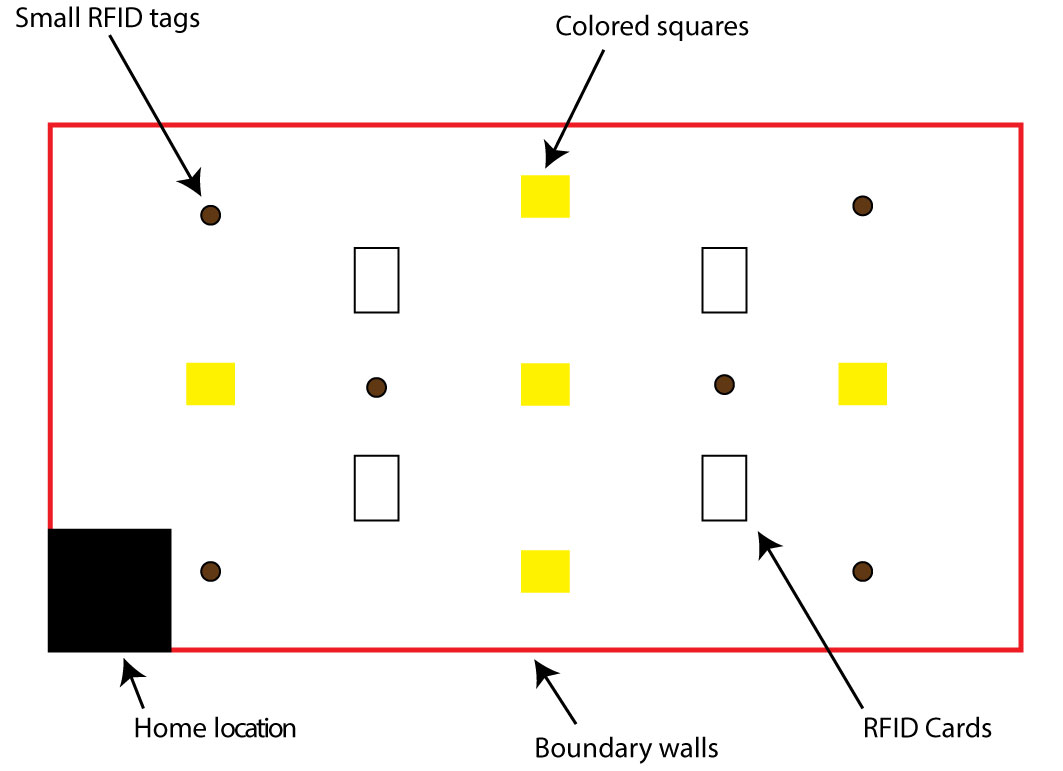
\includegraphics[width=1\columnwidth]{field.jpg}\\
%\caption{The test field is rectangular, with a solid black line for the robot to follow. The end of the black line is marked by a solid yellow square. The home location is designated by the solid black square in the lower left corner.}
%\label{F.field}
%\end{figure}

The hardware required for this challenge

The software design for this challenge 

\begin{equation}\label{E.motor_speed}
    P_{motor} = \frac{P_{max}-P_{min}}{I_{max}-I_{min}}I_{sensor} + offset
\end{equation}

\section{Problems Encountered}\label{S.problems}
This particular project was extremely challenging as we encountered numerous problems. 

First we needed to find a mechanism to acquire balls that met several criteria. The physical mechanism needed to be able to grasp a found ball, detect that a ball was successfully grasped, hold the ball for transport, and sucessfully deploy the ball over the side of the arena. 

The biggest problem during this project, however, was finding a strategy to find balls. This required a strategy for the robot to put itself into a position to approach the field on the end of the arena where the balls originated, searching for balls once there,approaching and capturing an individual ball once discovered, and deploying the ball to the appropriate end of the arena. 

\section{Solutions}\label{S.solutions}
We developed an incline on the front of the robot that would very reliably push a captured ball over the edge of the arena when the robot rolled toward the edge. This passive approach allowed us to employ a motor directly for the grasper, which would deploy over the incline very effectively capturing a ball on the incline. In order to identify the ball, we installed a color sensor on the grasper that would move with the grasper, allowing us the flexibility to have the sensor out of the way when the grasper was not deployed. 

We had developed a plan to use sonar sensors to identify balls in the field by making the robot rotate on a central axis and scan the field for balls with the sonar sensor. By sensing where relatively large and sudden changes in distance observed occured, the robot theoretically would be able to detect where a ball was and be distinuishable from the wall of the arena. By knowing the exact amount to rotate by (if the sensor is in a fixed position relative to the front of the robot) and the exact distance to travel (provided by the sensor), the robot would be able to turn and move forward toward the ball and grasp it. Unfortunately, this was never implemented. 

Instead, due to the large density of balls in the field, we employed the color sensor as a ball detector by lowering the resting position of the grasper and using a waddling action to move and sweep over the balls. This was mildly effective, as the robot would sometimes push balls out of the way and miss them entirely. This would break the robot's cycle of behavior and it would begin behaving unpredictably.

The robot's ability to distinguish balls and deploy them over the wall of the appropriate side of the field worked spectacularly thanks to the compass. The robot would be initialized by hand to tell it the direction of each end of the arena and then used to refine the motion of the robot in transit. The robot would drive toward the appropriate end of the field, raise the grapser while in motion so the ball rests against the incline, and then plow into the wall of the arena, ejecting the ball.

\section{Unsolved Problems}\label{S.unsolved}
Unfortunately, reliably discovering balls proved to be very difficult and our solution and implementation proved to be unreliable. 

\end{document}
